
\section{Website}\label{sec:website}

\renewcommand{\kapitelautor}{Autor: Irgendwer} % todo: replace

%
% text goes here
%

\subsection{Implementation}
\renewcommand{\kapitelautor}{Autor: Marvin Kurka}

Da es sich bei der Website um eine relativ simple, statische Website handelt, die kaum mit dem User interagiert wurde
die Entscheidung getroffen kein Framework wie \zB Vue oder React zu verwenden.
Allerdings wurde Sass verwendet, eine Css-Extension, die mehrere Features hat, die das Erstellen und Strukturieren
von großen Stylesheets vereinfachen.
Sass erlaubt \zB das Erstellen und Verwenden von Variablen, das Unterordnen von Selektoren oder das Aufteilen von
Stylesheets in mehrere Dateien.\cite{sassDoc}
Da ein relativ umfangreiches Stylesheet für die Website notwendig war, wurde die Entscheidung getroffen Sass zu
verwenden, um die Maintainability zu erhöhen.

Eine weitere Eigenschaft der \FF Website ist, dass besonders viele Bilder verwendet werden, um die Website dem Stil des
Spiels anzugleichen.

\begin{figure}[H]
    \centering
    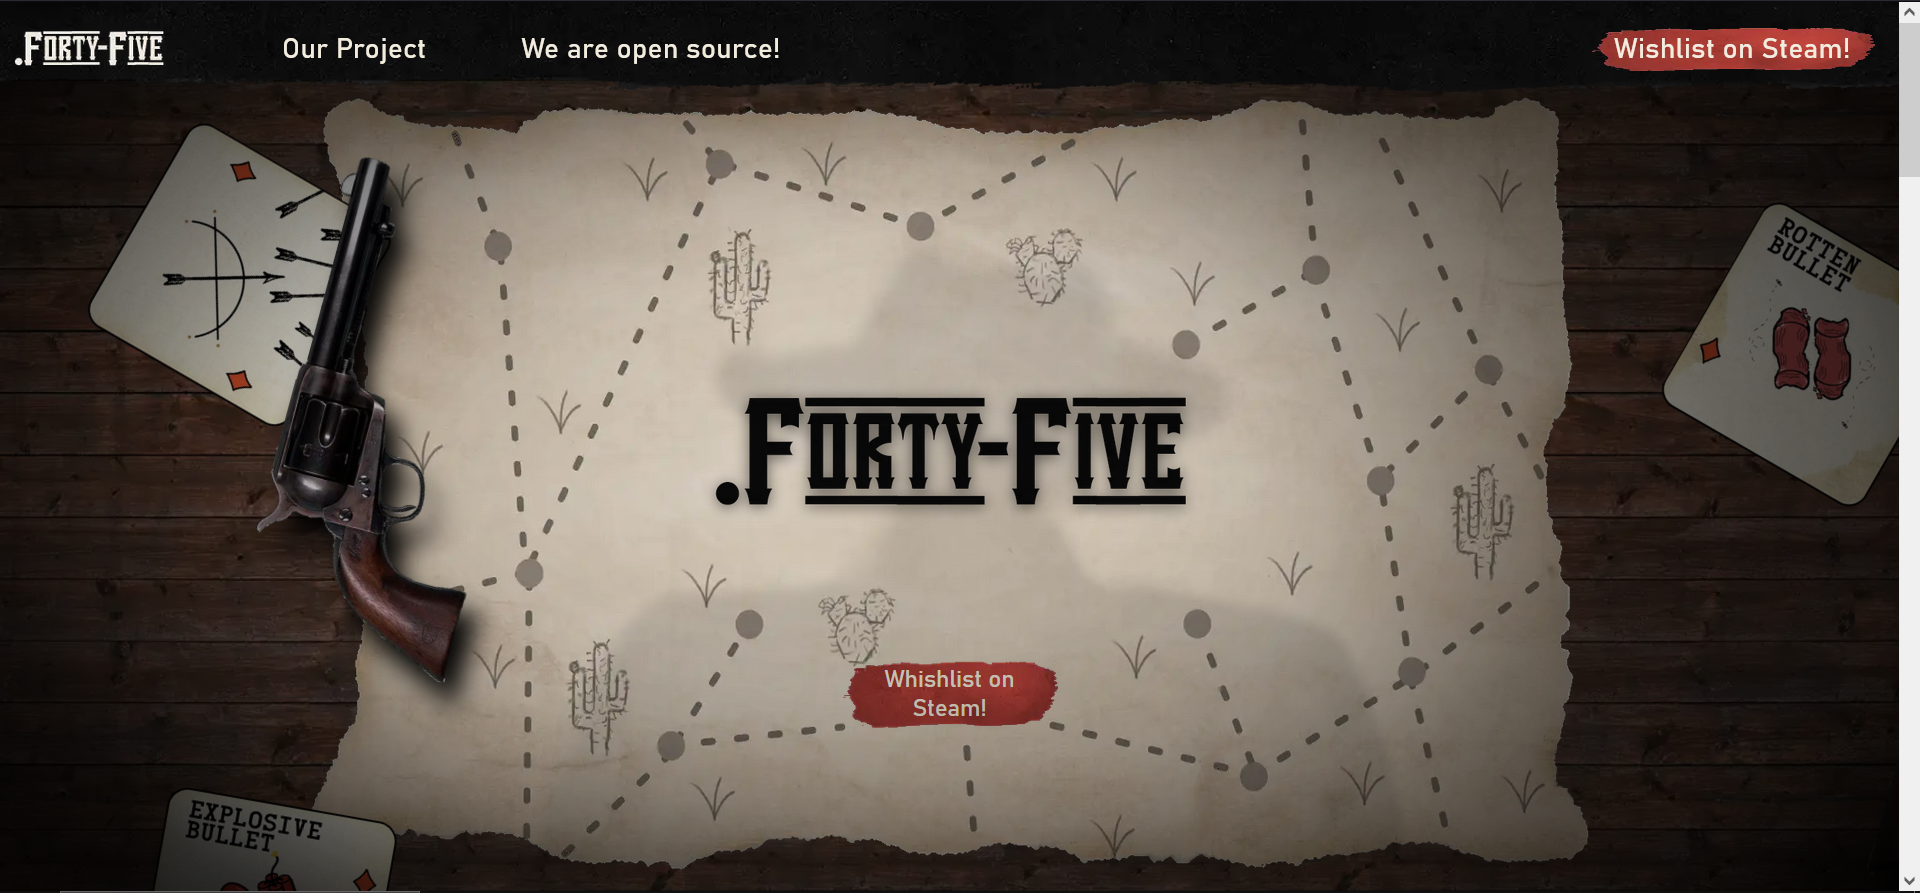
\includegraphics[width=1.0\textwidth]{website.png}
    \caption{Screenshot der Website}
\end{figure}

Das wirkt sich natürlich negativ auf die Ladezeiten der Website aus.
Um diesen Effekt so gering wie möglich zu halten, wurde das von Google entwickelte webp Bild-Format verwendet, welches
eine deutlich bessere Komprimierung als vergleichbare Formate wie \zB jpg erzielt.
In einer vergleichenden Studie, welche von Google durchgeführt wurde, erreichte webp je nach verwendeter Methodik eine
Verkleinerung von 14\% gegenüber eines mit jpg komprimierten Bildes.\cite{googleWebpStudie}

% resets author
\renewcommand{\kapitelautor}{}
